\begin{frame}
    \frametitle{LED}
    \begin{center}
        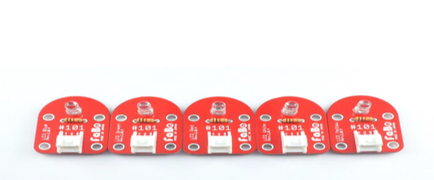
\includegraphics[width=0.8\textwidth]{images/chap05/text05-img016.png}
        \begin{itemize}
            \item 値が1のとき光る
            \item 値が0のとき消える
        \end{itemize}
    \end{center}
\end{frame}

\begin{frame}
    \frametitle{振動子(しんどうし)}
    \begin{center}
        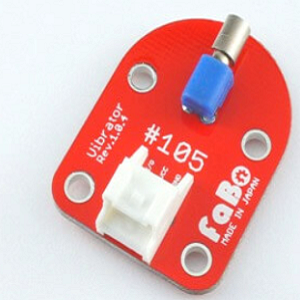
\includegraphics[width=0.4\textwidth]{images/chap05/text05-img017.png}
        \begin{itemize}
            \item 値が1のとき震(ふる)える
            \item 値が0のとき動かない
        \end{itemize}
    \end{center}
\end{frame}

\begin{frame}
    \frametitle{センサーをピンにつけてみよう}
    \begin{center}
        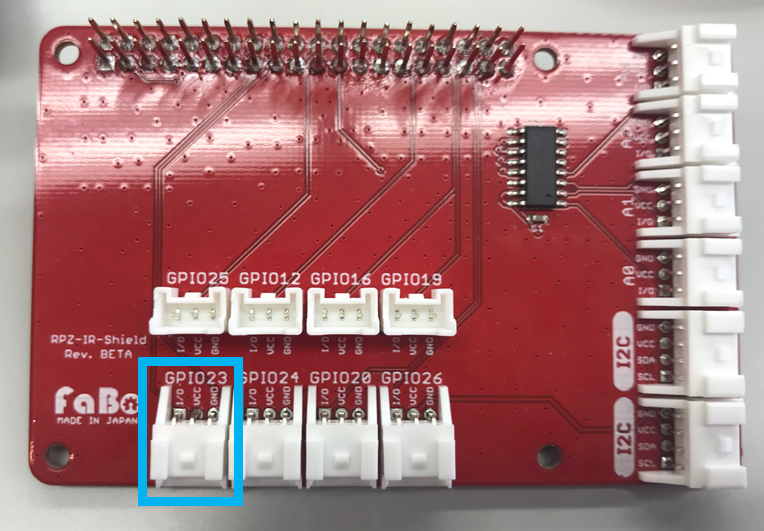
\includegraphics[width=0.4\textwidth]{images/chap05/text05-img027.png}
        \begin{itemize}
            \item GPIO23とLEDをつなげてみよう
            \item HSPでdigout.hspを動かしてみよう
        \end{itemize}
    \end{center}
\end{frame}

\begin{frame}[fragile]
    \frametitle{デジタル出力センサを使ったプログラム(digout.hsp)}
\begin{lstlisting}
#include "hsp3dish.as"
#include "rpz-gpio.as"

*main
    redraw 0
    font "",20
    pos 20,20
    mes "センサーが動いたり止まったりします"
    redraw 1

    gpio 23,1
    wait 100
    gpio 23,0
    wait 100
    goto *main
\end{lstlisting}
\end{frame}

\begin{frame}[fragile]
    \frametitle{問題を解いてみよう}
    \begin{itemize}
        \item 教科書13ページ 問題5-4
        \begin{itemize}
            \item 2問
        \end{itemize}
    \end{itemize}
\end{frame}